%% Preambulo, paquetes a cargar por compilador latex
\documentclass[12pt]{beamer}
\mode<presentation>{
  % selección de tema y color
  \usetheme{Copenhagen}
  \usecolortheme{orchid}
}

\usepackage[utf8]{inputenc}
\usepackage[spanish]{babel}
\usepackage{float}
\usepackage{graphicx}
\usepackage{caption}
\usepackage{subcaption}
\usepackage{verbatim}
\usepackage{url} 
\usepackage[export]{adjustbox}
\usepackage{listings}
\usepackage{tcolorbox}
\usepackage{tikz}
\usepackage{cclicenses}
\usepackage{multicol}
\lstdefinestyle{mystyle}{
  basicstyle=\tiny,
  language=Python
}
\lstset{style=mystyle}

%% Automatizar localización de las imágenes
\graphicspath{{./img/}}

\title{Introdución a Python, Git y Github}
\author[Fran Rúa/Breixo Camiña]{Fran Rúa \\ Breixo Camiña}
\institute[GPUL-Labs]{Grupo de Programadores e Usuarios Linux}
\date{\today}

\begin{document}

\begin{frame}
  \titlepage
  \begin{tcolorbox}[]
    \centering
    {\small \bysa}\\
    {\tiny Esta obra está suxeita á licencia
      Recoñecemento-CompartirIgual 4.0 Internacional de Creative
      Commons. Para ver unha copia desta licencia, visite
      http://creativecommons.org/licenses/by-sa/4.0/.}
  \end{tcolorbox}
\end{frame}

\begin{frame}
  \frametitle{Índice}
  \tableofcontents
\end{frame}

\usebackgroundtemplate{%
  \tikz[overlay,remember picture] 
  \node[opacity=0.3 , at=(current page.south east),anchor=south east] {
    
\includegraphics[]{logo-labs}};
}


\title[Python]{Introducción a Python}
\date{}
\author[Fran Rúa/Breixo Camiña]{}
\institute{}

\section{Python}
\label{sec:Python}

\usebackgroundtemplate{}
\begin{frame}
  \titlepage
  \begin{figure}[H]
    \centering
    
\includegraphics[scale=0.5]{python-logo}
  \end{figure}
\end{frame}

\usebackgroundtemplate{%
  \tikz[overlay,remember picture] 
  \node[opacity=0.3 , at=(current page.south east),anchor=south east] {
    
\includegraphics[]{logo-labs}};
}

\begin{frame}
  \frametitle{Fontes e referencias}
  \begin{itemize}
  \item Documentación oficial de Python\\
    {\color{blue}\url{www.python.org/doc}}
  \item Guías de estilo PEP\\
    {\color{blue}\url{www.python.org/dev/peps/pep-0008/}}
  \item Guía para principiantes\\
    {\color{blue}\url{wiki.python.org/moin/BeginnersGuide}}
  \item Learn Python (español)\\
    {\color{blue}\url{http://www.learnpython.org/es/}}
  \item Tracducción do manual de Guido van Rossum
    {\color{blue}\url{http://docs.python.org.ar/tutorial/pdfs/TutorialPython2.pdf}}
  \item Información adiccional\\
    {\color{blue}\url{s.wikipedia.org/wiki/Python}}
  \end{itemize}
\end{frame}

\subsection{Introducción}
\label{subsec:Introduccion}

\begin{frame}
  \frametitle{Introducción}
  \begin{itemize}
  \item Historia
  \item Para qué é usado.
  \item Características
  \item Ventaxas
  \item Inconvintes
  \end{itemize}
\end{frame}

\begin{frame}
  \frametitle{Historia}
  \begin{itemize}
  \item Creado a finais dos 80's por Guido van Rossum
  \item Desenvolvido para o SO Amoeba
  \item Toma partes de outros linguaxes de programación, como Haskell ou ABC
  \item A súa finalidade é programar facilmente e obrigar ó programador a
    realizar código entendible.
  \item Python 1.0 liberado en xaneiro de 1994
  \item Actualmente dous proxectos paralelos: Python 2.7 e Python 3.4
  \item Instalado por defecto na maioría das distribucións GNU/Linux
  \end{itemize}
\end{frame}

\begin{frame}
  \frametitle{Características}
  \begin{itemize}
  \item Linguaxe de programación interpretado
  \item Multiplataforma
  \item Multiparadigma (Programación imperativa, orientada a obxectos e funcional)
  \item Tipado dinámico
  \item Código aberto (Python Software Foundation License, compatible con GNU)
  \item Herencia
  \item Modo interactivo
  \end{itemize}
\end{frame}

\begin{frame}
  \frametitle{Para qué é usado}
  \begin{itemize}
  \item Inicialmente, tareas livianas ou de administración.
  \item Posúe unha ampla cantidade de librerías que posibilita un amplo rango
    de escenarios de uso
  \item Computación numérica
  \item Xeración de gráficos
  \item Programación web
  \item Interacción con bases de datos
  \item Programas de usuario con interface gráfico.
  \end{itemize}
\end{frame}

\subsection{Funcionamento}
\label{subsec:funcionamento}

\begin{frame}
  \frametitle{Funcionamento}
  Ó contrario que C ou Java, Python non precisa ser compilado. En realidade
  Python é un intérprete de comandos que acepta unha serie de instruccións que
  respetan unha serie de normas lóxicas e semánticas.

  Por tanto, se queremos executar o noso código en múltiples plataformas, só é
  necesario instalar o intérprete, xa que despois será éste o encargado de
  executar as órdes indicadas polas instruccións.
\end{frame}

\begin{frame}
  \frametitle{Compilación vs. Interpretación}
  \begin{figure}[ht]
    \centering
    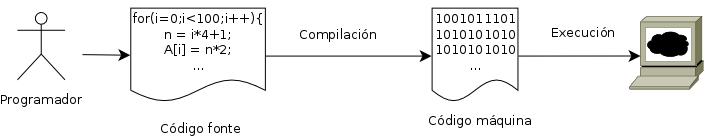
\includegraphics[scale=0.3]{compilacion.png}
    \caption{Compilacion de un programa}
  \end{figure}
\end{frame}

\begin{frame}
  \frametitle{Compilación vs. Interpretación}
  \begin{figure}[ht]
    \centering
    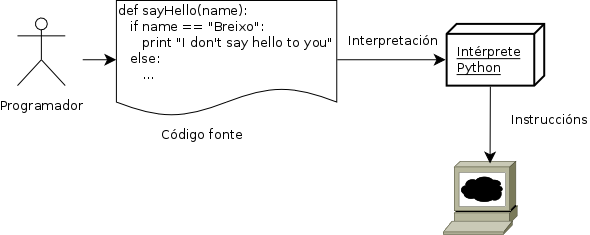
\includegraphics[scale=0.3]{interpretacion.png}
    \caption{Interpretacion de un programa}
  \end{figure}
\end{frame}

\subsection{Modo Interactivo}
\label{subsec:modo interactivo}

\begin{frame}
  \frametitle{Que é o modo interactivo?}
  O modo interactivo permítenos iniciar unha instancia do intérprete de python,
  o que nos permite programar en tempo real e comprobar a sintaxis do noso
  programa.
  
  Neste modo podemos cargar librerías e módulos, ee executar funcións de forma
  rápida sen necesidade de realizar programas previamente.
\end{frame}

\begin{frame}[fragile]
  \frametitle{Iniciar modo interactivo}
  Nos sistemas GNU/Linux soamente é necesario abrir un emulador do terminal e
  escribir \emph{python}.
  \small
\begin{verbatim}
[fran@izanami ~]$ python
Python 2.7.10 (default, Sep 24 2015, 17:50:09) 
[GCC 5.1.1 20150618 (Red Hat 5.1.1-4)] on linux2
Type "help", "copyright", "credits" or "license" for more information.
>>> 
\end{verbatim}
  \normalsize
\end{frame}

\begin{frame}
  \frametitle{Sair do modo interactivo}
  Unha vez que rematemos, para sair do modo iteractivo só temos que chamar á
  función \emph{exit()}

  As funcións e variables definidas nunha sesión do intérprete son borrados unha
  vez que se finaliza dita sesión.
\end{frame}

\subsection{Programando en Python}
\label{subsec:Programando}

\begin{frame}
  \frametitle{Tipos básicos}
  Os tipos de datos básicos definidos por Python son os seguintes:
  \begin{itemize}
  \item Enteiros (int)
  \item Numeros en punto flotante (float)
  \item Números longos (long)
  \item Números complexos (complex)
  \item Caracteres (char)
  \item Cadeas de caracteres (string)
  \item tuplas (tuple)
  \end{itemize}
\end{frame}

\begin{frame}
  \frametitle{Operadores lóxicos}
  \begin{itemize}
  \item and
  \item or
  \item not
  \item is, is not
  \item in, not in
  \end{itemize}
\end{frame}

\begin{frame}
  \frametitle{Operadores matemáticos}
  \begin{itemize}
  \item + (suma)
  \item - (resta)
  \item / (division)
  \item * (multiplicación)
  \item \% (módulo)
    % \item << >> (desplazamiento n bits a dereita ou esquerda)
  \end{itemize}
\end{frame}

\begin{frame}
  \frametitle{Estructuras de datos}
  Ademais dos tipos de datos básicos, Python soporta de forma nativa varias
  estructuras de datos, das cales veremos as dúas máis empregadas.
  \begin{itemize}
  \item \textbf{Listas}\\
    Conxunto de tipos básicos(enteiros, numeros en punto flotante) ou
    compostos(tuplas), poden estar ordenados ou non.\\
    a = [1,2,3,4]
  \item \textbf{Diccionarios}\\
    Asocian un valor a unha clave para mellorar o acceso a un determinado
    elemento.\\
    alumnos = \{'00001A':'Breixo','00002B':'Fran'\}
  \end{itemize}
\end{frame}

\begin{frame}[fragile]
  \frametitle{Definir variables}
  O intérprete python ten incorporado un motor de inferencia, o que significa
  que cando declaramos unha variable non temos que declarar o seu tipo, xa se
  encarga o propio intérprete de inferilo. Se temos dudas acerca do typo de unha
  variable, podemos sabelo coa función \emph{type()}
  \small
\begin{verbatim}
>>> sete = 7
>>> type(sete)
<type 'int'>
>>> a = "primeiro"
>>> type(a)
<type 'str'>
\end{verbatim}
  \normalsize  
\end{frame}

\begin{frame}[fragile]
  \frametitle{Funcións incorporadas (Built-in functions)}
  Python fai uso ten librerías por defecto, que non é necesario cargar, que
  proveen funcionalidades básicas, coma \emph{print()}, que aplicado sobre un
  tipo devolve a súa representación en caracteres.
  \small
\begin{verbatim}
>>> n = "cadea"
>>> print(n)
cadea
>>> numero = 745
>>> print(numero)
745
>>> flotante = 3.14
>>> print(flotante)
3.14
\end{verbatim}
  \normalsize   
\end{frame}

\begin{frame}
  \frametitle{Operacións sobre diccionarios}
  As operacións sobre direccionarios son proporcionados polas librerías básicas,
  xa que son un tipo moi empregado.
  \begin{itemize}
  \item Declaración\\
    d1 = {}
  \item Obter un elemento\\
    d1['clave']
  \item Engadir un elemento\\
    d1.update({'clave':'valor'})
  \item Borrar un elemento\\
    del d1['clave]
  \end{itemize}
\end{frame}

\begin{frame}
  \frametitle{Operacións sobre listas}
  Ó igual que os diccionarios, as listas tamén son moi empregadas e as
  operacións sobre estas son amplamente soportadas.
  \begin{itemize}
  \item Declaración\\
    l = []
  \item Obter un elemento por índice (comeza por 0)\\
    l[7]
  \item Engadir un elemento o final da lista\\
    l.append(n)
  \item Borrar un elemento i\\
    del l[i]
  \end{itemize}
\end{frame}

\begin{frame}[fragile]
  \frametitle{Definir funcións}
  Cando un fragmento de código é executado en numerosas ocasións, ou o código é
  extenso e complexo faise necesario estructuralo en funcións. En python as
  funcións declaranse da seguinte forma:
  \small
\begin{verbatim}
def <nome_funcion>(parametro1,parametro2,...,parametroN):
   sentencias dentro da función
\end{verbatim}  
  \normalsize
\end{frame}

\begin{frame}[fragile]
  \frametitle{Función de suma}
  \small
\begin{verbatim}
>>> def suma(a,b):
...    return a+b
... 
>>> suma(3,4)
7
\end{verbatim}
\end{frame}

\begin{frame}[fragile]
  \frametitle{Indentación}
  Como vimos ó principio, un dos obxectivos de Python é conseguir un código
  claro e lexible, para o cal fai obligatorio o uso da indentación.

  Unha mala indentación cambia o significado do programa.
  \begin{multicols}{2}
    \begin{lstlisting}
      def access_control(name, pass):
        if authentication(name,pass) == 0:
          print(``Access denied'')
          exit()
        else:
          print(``Access granted'')
          grant_access()
    \end{lstlisting}
    \columnbreak
    \begin{lstlisting}
      def access_control(name, pass):
        if authentication(name,pass) == 0:
          print(``Access denied'')
          exit()
        else:
          print(``Access granted'')
        grant_access()
    \end{lstlisting}
  \end{multicols}
\end{frame}

\begin{frame}[fragile]
  \frametitle{Estructuras de control}
  \framesubtitle{If}
  \small
  \begin{verbatim}
    if (test1):
       print a
    elif (test2 and test3):
       print b
       exit()
    elif (test4):
       print(``nada que facer'')
    else:
       print(``Saindo'')
  \end{verbatim}
  \normalsize
\end{frame}

\begin{frame}[fragile]
  \frametitle{Estructuras de control}
  \framesubtitle{Bucle for}
  Os bucles for son aplicados sobre listas. Esto quere decir que se queremos
  percorrer unha lista e aplicar unha función a cada elemento, ésto é posible
  mediante o seguinte código
  \small
\begin{verbatim}
>>> alumnos = ["Xoan", "Marcos","Jesus", "Bea"]
>>> for alumno in alumnos:
...    print alumno
... 
Xoan
Marcos
Jesus
Bea
>>> 
\end{verbatim}
  \normalsize
\end{frame}

\begin{frame}[fragile]
  \frametitle{Bucle for}
  Se queremos un bucle secuencial, podemos empregar a función \emph{range}, que
  crea unha lista de elementos.
  \small
  \begin{verbatim}
    >>> for n in range(2,8):
    ...    print n
    ... 
    2
    3
    4
    5
    6
    7
    >>> 
  \end{verbatim}
  \normalsize
\end{frame}

\begin{frame}[fragile]
  \frametitle{Estructuras de control}
  \framesubtitle{Bucle while}
  Igual que no resto de linguaxes de programación, o bucle while permítenos
  realizar unha acción repetitiva mentrs se cumpla unha condición, usando a a
  sentencia \textbf{break} para saír. Se non queremos saír do bucle, senón
  saltar as sentencias pendentes e executar o seguinte salto de bucle usamos
  \textbf{continue}.
  \small
\begin{verbatim}
    while(true):
       if(test1):
          continue
       elif(test2):
          print("Hola")
       else:
          break    
\end{verbatim}
  \normalsize
\end{frame}

\begin{frame}
  \frametitle{Ficheiros de código}
  Python é un programa de scripting, é decir, as instruccións son escritas nun
  ficheiro de texto plano, con extensión \emph{.py} tal e como serían
  introducidas no intérprete.  

  A execución de un script consiste básicamente na lectura secuencial do
  ficheiro de texto e a execución das insctruccións correspondentes por parte do
  intérprete. 

  Existen dous tipos de programar en ficheiros: módulos e programas.
\end{frame}

\begin{frame}
  \frametitle{Módulos}
  Os módulos son definicións de funcións. Se existen funcións que usamos
  reiteradamente, podemos definilas nun ficheiro con extensión \emph{.py} e
  importalo despois mediante a orde \textbf{import}.

  Os módulos proporcionan funcionalidades, pero non realizan accións de por sí,
  senon que son usados polos programas para axilizar o desenvolvemento de
  aplicacións. 

  Existen dúas formas de referenciar módulos, \textbf{import} e \textbf{from}
\end{frame}

\begin{frame}[fragile]
  \frametitle{Modulo operacions.py}
  \small
  \begin{verbatim}
    def suma (a,b):
        return a+b
    
    def resta (a,b):
        return a-b

    def devolve_maior (a,b):
        if (a>b):
            return a
        else:
            return b
  \end{verbatim}
  \normalsize
\end{frame}

\begin{frame}[fragile]
  \frametitle{import}
  A sentencia \textbf{import} carga todas as funcións do módulo ó que
  referenciamos, o cal pode ser ineficiente se non as empregamos.

  Ademáis, o programador debe especificar o espazo de nomes, é decir,
  referenciar o módulo ó que pertence a función que queremos empregar.

  \small
  \begin{verbatim}
>>> import operacions
>>> suma(2,8)
Traceback (most recent call last):
  File "<stdin>", line 1, in <module>
NameError: name 'suma' is not defined
>>> operacions.suma(2,8)
10
  \end{verbatim}  
  \normalsize
\end{frame}

\begin{frame}[fragile]
  \frametitle{from}
  Mediante a orde \textbf{from}, podemos importar funcións concretas de un
  módulo e, ademáis, importar o seu espazo de nomes, polo que non é necesario
  facer referencia ó módulo ó que pertence.
  \small
  \begin{verbatim}
>>> from operacions import devolve_maior
>>> devolve_maior(15,8)
15
>>> operacions.devolve_maior(15,8)
Traceback (most recent call last):
  File "<stdin>", line 1, in <module>
NameError: name 'operacions' is not defined
  \end{verbatim}
  \normalsize
\end{frame}

\begin{frame}
  \frametitle{Scripts Python}
  Obviamente é interesante ter programas que se executen de forma que non sexa
  necesario o uso de unha sesión interactiva co intérprete. A estes ficheiros
  denomínase scripts, e, ó igual que os módulos, son leidos polo intérprete de
  forma secuencial.

  Neles podemos definir un conxunto de funcións e variables coas que construir
  unha secuencia de pasos a executar.

  Para que se execute é necesario que exista unha función \textbf{main}, que é a
  última en ser declarada.

  Cando o intérprete lee un arquivo de texto, se existe unha función main
  executa as ordes dentro dela como si se tratara dunha sesión interactiva, de
  forma que pode ser usada como disparador de un conxunto de accións.
\end{frame}

\begin{frame}[fragile]
  \frametitle{Cabeceiras}
  Para executar un programa en python, tan só é necesario asegurarnos de que o
  arquivo ten permisos de execución e a continuación chamar ó interprete sobre o
  ficheiro.
  \small
  \begin{verbatim}
    python arquivo.py
  \end{verbatim}
  \normalsize
  É posible engadir a seguinte liña para que o script sexa executado polo propio
  entorno de usuario.
  \small
  \begin{verbatim}
    #!/usr/bin/env python 
  \end{verbatim}
  \normalsize
  Tamén é recomendable, se o texto vai incluir carácteres que poden ser
  problemáticos coma 'ñ', ou tildes, especificar a codificación na que se gardou
  o ficheiro. O máis apropiado é facelo en UTF-8
  \begin{verbatim}
    # -*- coding: utf-8 -*-
  \end{verbatim}
  \normalsize
\end{frame}

\begin{frame}
  \frametitle{Inconvintes}
  \begin{itemize}
  \item Os erros teñen lugar en tempo de execución
  \item Como o tipado é dinamico, require que o programador preste maior
    atención a estos detalles.
  \item Rendemento, principalmente na carga de código
  \end{itemize}
\end{frame}
              % introducción a python
% !TeX spellcheck = es_ES

% Funcionamento e uso de un CVS: Git
\title[Git e GitHub]{Control de versións Git}
\author[Fran Rúa e Breixo Camiña]{}

\section{Control de versións Git}
\label{sec:Git}

\begin{frame}
  \titlepage
	\begin{figure}[H]
	\centering
	
\includegraphics[width=0.5\linewidth]{./img/logo-git}
	\label{fig:logo-git}
	\end{figure}
\end{frame}

\begin{frame}
	\frametitle{Táboa de contidos}
	\tableofcontents[currentsection]
\end{frame}

\subsection{Sistema de control de versións}
\label{subsec:vcs}
\begin{frame}{Sistema de control de versións}
\begin{block}{¿Que é o control de versións?}
	É a xestión de diversos cambios que se realizan sobre os elementos de algún produto ou unha configuración do mesmo. Unha versión é o estado no que se encontra o produto nun momento do seu desenvolvemento.
\end{block}
	\begin{block}{¿Que é un sistema de control de versións?}
		Son ferramentas que facilitan a administración das distintas versións de cada produto desenvolvido.
	\end{block}
\end{frame}

\subsection{¿Que é Git?}
\begin{frame}
  \frametitle{¿Que é Git?}
  \begin{block}{Definición}
	  Git é un sistema de control de versións distribuido gratuito e de código aberto deseñado para xestionar todo dende un proxecto pequeno a un moi grande, de forma rápida e eficiente.
  \end{block}
  \begin{itemize}
	  \item É rápido, eficiente, escalable e distribuido.
	  \item Propicia o traballo en local e o uso de ramas.
	  \item Proporciona un nivel de historia do proxecto completísimo.
	  \item Diferencia os commits unívocamente mediante claves xeradas con SHA-1.
	  \item Cumpre as palabras máxicas do GPUL: é libre e gratuito.
  \end{itemize}
\end{frame}

\subsection{Comparación con outros servizos}
\begin{frame}
	\scriptsize
  	\frametitle{Comparación con servizos de almacenamento na nube}
	\begin{multicols}{2}
	 \textbf{Dropbox:}
	 \begin{itemize}
	  \item Útiles para compartir ficheiros con compañeiros.
	  \item O problema é se queres modificar o mesmo ficheiro ambos ó mesmo tempo, vai haber problemas de sincronización.
	 \end{itemize}
		\columnbreak
	 \textbf{Google Drive:}
	 \begin{itemize}
	  \item Útil para modificar ficheiros en tempo real, pero con proxectos software é imposible.
	 \end{itemize}
	\end{multicols}
	\begin{alertblock}{VCS}
	  	Os VCS son a solución!
	\end{alertblock}
\end{frame}

\begin{frame}
	\frametitle{Comparación con outros VCS}
	\tiny
	\begin{multicols}{2}
		 \textbf{Subversion:}
		 \begin{itemize}
		 	\item Git é moito máis rápido e lixeiro que SVN (un repo SVN ocupa 30x o que un de Git).
			\item Unha rama en SVN é unha copia completa do repositorio mentres que en Git é un simple punteiro e conleva toda a historia do proxecto ata ese punto.
			\item Git proporciona mellor auditoría de eventos de ramificación e fusión (ramas e merge).
			\item SVN é usado en case todas as asignaturas da FIC.
			\item Por dicir algo bo de SVN, é máis fácil o seu uso para principiantes e ten máis ferramentas de integración con IDEs.
		 \end{itemize}
		\begin{figure}
			\centering
			
\includegraphics[width=0.3\linewidth]{./img/svn}
			\label{fig:svn}
		\end{figure}

		\columnbreak

		 \textbf{Mercurial:}
		 \begin{itemize}
		  \item Máis fácil de aprender que Git.
		  \item Mercurial blablabla
		 \end{itemize}
		\begin{figure}
		\centering
		
\includegraphics[width=0.3\linewidth, height=0.2\textheight]{./img/mercurial}
		\label{fig:mercurial}
		\end{figure}
		\end{multicols}
\end{frame}

\subsection{Instalación nos SO}
\begin{frame}
	\frametitle{Instalación nos SO}
	\begin{exampleblock}{Linux}
		(Proyecto Debian) apt-get install git\\
		(RPM) yum install git
	\end{exampleblock}
	\begin{block}{Mac}
		http://git-scm.com/download/mac
	\end{block}
	\begin{alertblock}{Windows}
		https://git-scm.com/download/win
	\end{alertblock}	
\end{frame}

\begin{frame}
	\frametitle{Interfaces gráficas de usuario para Git}
	\begin{exampleblock}{Linux}
			SmartGit - http://www.syntevo.com/smartgit/download
		\end{exampleblock}
		\begin{alertblock}{Mac e Windows}
			Sourcetree - https://es.atlassian.com/software/sourcetree/overview/
		\end{alertblock}
\end{frame}

\subsection{Inicio do uso de Git}
\begin{frame}[fragile]
	\frametitle{Inicio do uso de Git}
	\small
	Creamos unha carpeta no escritorio que lle chamaremos "CharlaGit".
	Dentro da carpeta, executamos \textbf{git init} e debería saír:
	\tiny
	\begin{verbatim}
	breixocf@BreixoCF ~/Desktop/PruebasGit 6 $ git init 
	Initialized empty Git repository in /home/breixocf/Desktop/CharlaGit/.git/
	\end{verbatim}
	\small
	Creouse unha carpeta .git que conterá todo o repositorio, que será a base de datos de Git.
	Antes de nada, imos configurar o noso repo, indicando o nome e correo do usuario con \textbf{git config}  e comprobamos os cambios.
	\tiny
	\begin{verbatim}
	breixocf@BreixoCF ~/Desktop/CharlaGit 18 $ git config --global user.name "Breixo Camiña"
	breixocf@BreixoCF ~/Desktop/CharlaGit 19 $ git config --global user.email 
	breixocf@BreixoCF ~/Desktop/CharlaGit 21 $ git config --list 
	user.name=Breixo Camiña
	user.email=breixo.camina@udc.es
	core.repositoryformatversion=0
	core.filemode=true
	core.bare=false
	core.logallrefupdates=true
	\end{verbatim}	
\end{frame}

\begin{frame}[fragile]
	\frametitle{Zonas de traballo de Git}
	\begin{multicols}{2}
		\begin{figure}
		\centering
		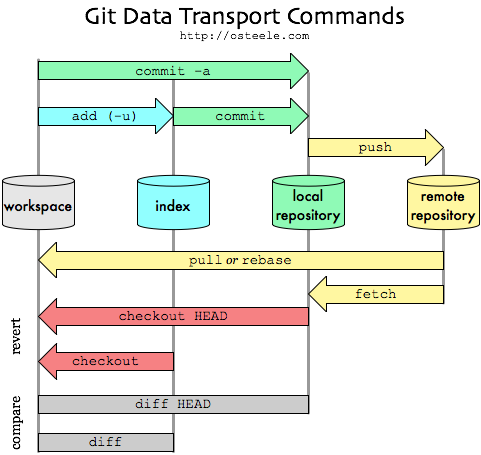
\includegraphics[width=1\linewidth]{./img/flujo-git}
		\label{fig:flujo-git}
		\end{figure}
		\columnbreak
		\tiny
		\begin{itemize}
			\item Workspace: É onde están os ficheiros que actualmente non están en seguimento, é dicir, os que están na nosa zona de traballo.
			\item Index: É onde están as modificacións que se engadirán ó repo local. Os ficheiros están preparados para engadir ó repositorio local, pero aínda non están no historial do proxecto. 
			\item Local Repository: É onde están os ficheiros confirmados que conformarán unha versión nova do proxecto. Almacena os metadatos e a base de datos do proxecto. Tamén se lle chama HEAD.
			\item Remote Repository: Son os repositorios que estarán en internet, onde accederán varios usuarios...
		\end{itemize}
	\end{multicols}
\end{frame}

\begin{frame}[fragile]
	\frametitle{Primer comando: git status}
	\begin{block}{git status}
		Amosa o estado no que se atopan os ficheiros do repositorio.
	\end{block}
	Executando \textbf{git status} sobre o noso repositorio, debería aparecer a seguinte mensaxe:
	\tiny
	\begin{verbatim}
	breixocf@BreixoCF ~/Desktop/CharlaGit 32 $ git status
	On branch master
	Initial commit
	nothing to commit (create/copy files and use "git add" to track)
	\end{verbatim}
	\small Como todavía non hai ningún ficheiro en seguimento (pode haber milleiros de ficheiros na carpeta, pero non están sendo trackeados polo repositorio), dinos que usemos git add para engadir algún ficheiro a seguir.
\end{frame}

\begin{frame}[fragile]
	\frametitle{Segundo comando: git add}
	\begin{block}{git add}
		Engade un ficheiro da nosa zona de traballo ao índice, preparándoo para engadilo ao seguimento.
	\end{block}
	\small
	Creamos un ficheiro co comando \textbf{touch hola.txt} e executamos \textbf{git status} para ver o seu estado:
	\tiny
	\begin{verbatim}
	breixocf@BreixoCF ~/Desktop/CharlaGit 32 $ git status
	On branch master
	Initial commit
	Untracked files:
	  (use "git add <file>..." to include in what will be committed)
	     hola.txt
	nothing added to commit but untracked files present (use "git add" to track)
	\end{verbatim}
\end{frame}

\begin{frame}[fragile]
	\frametitle{Segundo comando: git add}
	O ficheiro non está en seguimento pese a estar na carpeta, é necesario executar o comando \textbf{git add} para iso. Así que agora executamos \textbf{git add} e indicamos o ficheiro que queremos engadir. Se queremos engadir moitos ficheiros ó mesmo tempo, executamos \textbf{git add .}
	\tiny 
	\begin{verbatim}
	breixocf@BreixoCF ~/Desktop/CharlaGit 37 $ git add hola.txt 
	breixocf@BreixoCF ~/Desktop/CharlaGit 38 $ git status
	On branch master
	Initial commit
	Changes to be committed:
 (use "git rm --cached <file>..." to unstage)
	
		new file:   hola.txt
	\end{verbatim}
	\small
	Agora o ficheiro está preparado para engadir ó repo local.
\end{frame}

\begin{frame}[fragile]
	\frametitle{Terceiro comando: git commit}
	\begin{block}{git commit}
		Comando que serve para engadir ficheiros en seguimento (índice) ao repositorio local.
	\end{block}
	\small
	Executamos \textbf{git commit} para engadir ao repositorio o ficheiro \textit{hola.txt}. Para iso executamos \textbf{git commit -m "mensaxe"}. É importante que as mensaxes dos commits sexan precisos para que cando vexamos o histórico sepamos que fixemos en cada commit.
	\tiny 
	\begin{verbatim}
	breixocf@BreixoCF ~/Desktop/CharlaGit 39 $ git commit -m "Primeira subida do repositorio local"
	[master (root-commit) 7e8aa0a] Primeira subida do repositorio local
	 1 file changed, 0 insertions(+), 0 deletions(-)
	 create mode 100644 hola.txt
	breixocf@BreixoCF ~/Desktop/CharlaGit 40 $ git status
	On branch master
	nothing to commit, working directory clean
	\end{verbatim}
	\small
	Agora o ficheiro está no repo local.
\end{frame}

\begin{frame}[fragile]
	\frametitle{Terceiro comando: git commit}
	\scriptsize
	Imos crear máis ficheiros, concretamente \textit{atalogo.txt} e \textit{benvidos.txt}, do mesmo xeito que antes.
	Para comprobar os estados dos ficheiros, primeiro fago un git status, logo poño en seguimento o ficheiro atalogo.txt e volvo facer un status para que vexades como funciona:
	\tiny 
	\begin{verbatim}
	breixocf@BreixoCF ~/Desktop/CharlaGit 43 $ git status
	On branch master
	Untracked files:
	  (use "git add <file>..." to include in what will be committed)
		atalogo.txt
		benvidos.txt
	nothing added to commit but untracked files present (use "git add" to track)
	breixocf@BreixoCF ~/Desktop/CharlaGit 44 $ git add atalogo.txt 
	breixocf@BreixoCF ~/Desktop/CharlaGit 45 $ git status
	On branch master
	Changes to be committed:
	  (use "git reset HEAD <file>..." to unstage)
		new file:   atalogo.txt
	Untracked files:
	  (use "git add <file>..." to include in what will be committed)
		benvidos.txt
	\end{verbatim}
	\scriptsize
	Como podedes ver, o ficheiro \textit{benvidos.txt} segue sen estar en seguimento pero \textit{atalogo.txt} xa está en zona de preparación para 'commitear'. 
\end{frame}

\begin{frame}[fragile]
	\frametitle{Terceiro comando: git commit}
	\scriptsize
	Engadimos todos os ficheiros do repositorio (so debería estar pendente \textit{benvido.txt}) e facemos un novo commit cos dous ficheiros recién creados.
	\tiny 
	\begin{verbatim}
	breixocf@BreixoCF ~/Desktop/CharlaGit 46 $ git add .
	breixocf@BreixoCF ~/Desktop/CharlaGit 47 $ git status
	On branch master
	Changes to be committed:
	  (use "git reset HEAD <file>..." to unstage)
	
		new file:   atalogo.txt
		new file:   benvidos.txt
	
	breixocf@BreixoCF ~/Desktop/CharlaGit 48 $ git commit -m "Engadimos os ficheiros atalogo.txt e benvidos.txt"
	[master ce15277] Engadimos os ficheiros atalogo.txt e benvidos.txt
	 2 files changed, 0 insertions(+), 0 deletions(-)
	 create mode 100644 atalogo.txt
	 create mode 100644 benvidos.txt
	breixocf@BreixoCF ~/Desktop/CharlaGit 49 $ git status
	On branch master
	nothing to commit, working directory clean
	
	\end{verbatim}
	\scriptsize 
\end{frame}

\begin{frame}[fragile]
	\frametitle{Cuarto comando: git log}
	\begin{block}{git log}
	Este comando serve para ver o historial do repositorio.
	\end{block}
	\scriptsize
	Imos comprobar como está o noso historial de commits. Para eso executamos \textbf{git log}. Se non precisamos tanta información e queremos ver simplemente as mensaxes de cada commit executamos \textbf{git log - -oneline}.
	\tiny 
	
	\begin{multicols}{2}
	\begin{verbatim}
		breixocf@BreixoCF ~/Desktop/CharlaGit 50 $ git log
		commit ce152774dcba40748cfb8f1c622484ee89e87825
		Author: Breixo Camiña <breixo.camina@udc.es>
		Date:   Tue Feb 9 04:41:39 2016 +0100
		    Engadimos os ficheiros ...
		
		commit 7e8aa0a63c677bc789824e494fba7549b108246d
		Author: Breixo Camiña <breixo.camina@udc.es>
		Date:   Tue Feb 9 04:26:02 2016 +0100
		    Primeira subida do repositorio local
		    
		breixocf@BreixoCF ~ 51 $ git log --oneline
		ce15277 Engadimos os ficheiros ...
		7e8aa0a Primeira subida do repositorio local
		\end{verbatim}
		\columnbreak
		\tiny 
		\begin{itemize}
		\item git log --oneline --graph --all
		\item git log --oneline --graph --all --decorate
		\item git log --oneline --since=2016-02-01
		\item git log --oneline --until=2016-02-14
		\item git log --oneline --author="Breixo *"
		\item git log --oneline --grep="hola.txt"
		\item git log --stat --summary
		\end{itemize}
	\end{multicols}
	
\end{frame}

\begin{frame}[fragile]
	\frametitle{Modificando os ficheiros}
	\scriptsize
	Imos modificar agora os ficheiros a ver qué sucede no repositorio... Engadimos algún texto no ficheiro \textit{hola.txt} executando \textbf{echo "Hola a todos" \guillemotright hola.txt}.
	\tiny 
	\begin{verbatim}
	breixocf@BreixoCF ~/Desktop/CharlaGit 52 $ echo "Hola a todos" >> hola.txt 
	breixocf@BreixoCF ~/Desktop/CharlaGit 53 $ git status
	On branch master
	Changes not staged for commit:
	  (use "git add <file>..." to update what will be committed)
	  (use "git checkout -- <file>..." to discard changes in working directory)
	
		modified:   hola.txt
	
	no changes added to commit (use "git add" and/or "git commit -a")
	breixocf@BreixoCF ~/Desktop/CharlaGit 54 $ git add .
	breixocf@BreixoCF ~/Desktop/CharlaGit 55 $ git status
	On branch master
	Changes to be committed:
	  (use "git reset HEAD <file>..." to unstage)
	
		modified:   hola.txt
	\end{verbatim}
	\scriptsize 
	Como podedes ver, o ficheiro ó estar modificado temos que volver a engadilo para pasalo da zona de traballo á zona de preparación.
\end{frame}

\begin{frame}[fragile]
	\frametitle{Modificando os ficheiros}
	\scriptsize
	Engadímos o ficheiro e modificamos os outros dous do mesmo xeito. Comprobamos o estado:
	\tiny 
	\begin{verbatim}
	breixocf@BreixoCF ~/Desktop/CharlaGit 56 $ echo "Benvidas/os todas/os" >> benvidos.txt
	breixocf@BreixoCF ~/Desktop/CharlaGit 57 $ echo "Marcho que teño que marchar" >> atalogo.txt
	breixocf@BreixoCF ~/Desktop/CharlaGit 58 $ git status
	On branch master
	Changes to be committed:
	  (use "git reset HEAD <file>..." to unstage)
	
		modified:   hola.txt
	
	Changes not staged for commit:
	  (use "git add <file>..." to update what will be committed)
	  (use "git checkout -- <file>..." to discard changes in working directory)
	
		modified:   atalogo.txt
		modified:   benvidos.txt
	\end{verbatim}
	\scriptsize 
	Agora os tres ficheiros están modificados, pero \textit{hola.txt} está na zona de preparación listo para commitear mentres que \textit{atalogo.txt} e \textit{benvidos.txt} seguen na zona de traballo.
\end{frame}

\begin{frame}[fragile]
	\frametitle{Modificando os ficheiros}
	\scriptsize
	Engadimos os dous ficheiros á zona de preparación, comprobamos o estado do repo, facemos commit, volvemos comprobar o estado do repo e miramos o log do historial.
	\tiny 
	\begin{verbatim}
	breixocf@BreixoCF ~/Desktop/CharlaGit 60 $ git add .
	breixocf@BreixoCF ~/Desktop/CharlaGit 58 $ git status
	On branch master
	Changes to be committed:
 		(use "git reset HEAD <file>..." to unstage)
	
		modified:   hola.txt
		modified:   atalogo.txt
		modified:   benvidos.txt
		
	breixocf@BreixoCF ~/Desktop/CharlaGit 61 $ git commit -m "Engadimos texto nos 3 ficheiros"
	[master fec23c8] Engadimos texto nos 3 ficheiros
	 3 files changed, 3 insertions(+)
	breixocf@BreixoCF ~/Desktop/CharlaGit 63 $ git status
	On branch master
	nothing to commit, working directory clean
	breixocf@BreixoCF ~/Desktop/CharlaGit 62 $ git log --oneline
	fec23c8 Engadimos texto nos 3 ficheiros
	ce15277 Engadimos os ficheiros atalogo.txt e benvidos.txt
	7e8aa0a Primeira subida do repositorio local
	\end{verbatim}
\end{frame}

\begin{frame}[fragile]
	\frametitle{Quinto comando: git diff}
	\begin{block}{git diff}
		Este comando serve para ver as diferencias entre dous commits, un commit e o workspace...
	\end{block}
	\tiny
	Se executamos \textbf{git diff} agora, non vai haber ningunha diferencia, porque o workspace contén o mesmo que o último commit. Sen embargo, se engadimos un cambio nalgún documento con \textbf{echo "Hola por segunda vez a todos" \guillemotright hola.txt} e executamos \textbf{git diff} veremos o que ocorre. Se quixésemos ver os cambios dun arquivo concreto, simplemente teríamos que indicar qué arquivo sería executando \textbf{git diff hola.txt}. Para ver as diferencias entre a miña zona de preparación e o último commit, terías que executar \textbf{git diff --staged} e para ver as diferencias entre o workspace e o último commit, \textbf{git diff HEAD}.
	\tiny 
	\begin{verbatim}
	breixocf@BreixoCF ~/Desktop/CharlaGit 4 $ git diff
	breixocf@BreixoCF ~/Desktop/CharlaGit 5 $ echo "Hola por segunda vez a todos" >> hola.txt
	breixocf@BreixoCF ~/Desktop/CharlaGit 6 $ git diff
	diff --git a/hola.txt b/hola.txt
	index 1218745..384efad 100644
	--- a/hola.txt
	+++ b/hola.txt
	@@ -1 +1,2 @@
	 Hola a todos, son Breixo e o animaliño con roupa que teño ó lado Fran
	+Hola por segunda vez a todos
	\end{verbatim}
\end{frame}

\begin{frame}[fragile]
	\frametitle{Sexto comando: git tag}
	\begin{block}{git tag}
		Este comando serve etiquetar os snapshots ou releases que se quixeran facer.
	\end{block}
	\tiny
	Recoméndase crear etiquetas para cada versión funcional dun proxecto. Hai dous tipos de tags: simples e anotados. Un tag simple créase executando \textbf{git tag v1.0} mentres que un tag anotado crearíase executando \textbf{git tag -a v1.0 -m "Versión 1.4 do proxecto"}. Con \textbf{git tag}, amósase o listado de todos os tags do proxecto. Para mostrar info dun único tag executaríase \textbf{git show v1.0} e se quixéramos buscar por un patrón sería \textbf{git tag -l "v1.*"}.
	\tiny 
	\begin{verbatim}
	breixocf@BreixoCF ~/Desktop/CharlaGit 13 $ git tag v1.0
	breixocf@BreixoCF ~/Desktop/CharlaGit 14 $ git tag -a v1.1 -m "Versión 1.1"
	breixocf@BreixoCF ~/Desktop/CharlaGit 15 $ git tag 
	v1.0
	v1.1
	breixocf@BreixoCF ~/Desktop/CharlaGit 17 $ git show v1.0 
	commit 621a67beb491ecb02da730c0fcc866d73df7d2a3
	Author: Breixo Camiña <breixo.camina@udc.es>
	Date:   Wed Feb 10 00:56:37 2016 +0100
	    Engadida segunda liña no ficheiro hola.txt
	diff --git a/hola.txt b/hola.txt
	index 1218745..384efad 100644
	--- a/hola.txt
	+++ b/hola.txt
	\end{verbatim}
	\tiny
\end{frame}

\begin{frame}
	\frametitle{Séptimo comando: git checkout}
	\begin{block}{git checkout}
		Este comando serve para volver a pasos anteriores en ficheiros, commits ou ramas (prox.) pero só veremos nos dous primeiros.
	\end{block}
	\normalsize
	Executando \textbf{git checkout commit-id hola.txt}, o ficheiro hola.txt volve ó estado no que se atopaba nese commit. Mentres que se executas \textbf{git checkout commit-id}, todos os ficheiros volverían ó estado no que estaban nese commit.
	\tiny 
\end{frame}


\subsection{Repositorio remoto}
\begin{frame}
	\begin{figure}
	\centering
	\label{fig:github}
	
\includegraphics[width=0.7\linewidth, height=0.7\textheight]{./img/github}
	\end{figure}
\end{frame}

\begin{frame}[fragile]
	\frametitle{Repositorio remoto}
	\scriptsize
	Para crear o noso repositorio remoto, antes crearemos unha conta en GitHub. Logo de rexistrarnos, creamos un repositorio novo (New repository). Logo de indicarlle o nome, seguiremos os pasos que nos indican. Como xa temos o noso repositorio creado, con commits xa feitos sobre ficheiros, simplemente executaremos \textbf{git remote add origin https://github.com/BreixoCF/charlagit.git} e posteriormente faremos \textbf{git push -u origin master}.
	\tiny
	\begin{verbatim}
	breixocf@BreixoCF ~/Desktop/CharlaGit 19 $ git remote add origin 
	https://github.com/BreixoCF/charlagit.git
	breixocf@BreixoCF ~/Desktop/CharlaGit 20 $ git push -u origin master 
	Username for 'https://github.com': breixocf
	Password for 'https://breixocf@github.com': 
	Counting objects: 13, done.
	Delta compression using up to 4 threads.
	Compressing objects: 100% (9/9), done.
	Writing objects: 100% (13/13), 1.14 KiB | 0 bytes/s, done.
	Total 13 (delta 2), reused 0 (delta 0)
	To https://github.com/BreixoCF/charlagit.git
	 * [new branch]      master -> master
	Branch master set up to track remote branch master from origin.
	\end{verbatim}	
\end{frame}

\begin{frame}[fragile]
	\scriptsize
	Agora copiaremos este código dunha pila en Python nun ficheiro que chamaremos \textbf{stack.py}:
	\tiny
	\begin{verbatim}
	# Implementación de unha pila facendo uso de programacion orientada a obxectos.
	class Stack:
	    def __init__(self):
	        self.items = []
	
	    def vacia(self):
	        return self.items == []
	
	    def apilar(self, item):
	        self.items.append(item)
	
	    def cima(self):
	        if self.vacia():
	            return []
	        return self.items[-1]
	
	    def desapilar(self):
	        del self.items[-1]
	
	    def tam(self):
	        return len(self.items)
	\end{verbatim}
\end{frame}

\begin{frame}
	\normalsize
	Agora imos a subir o ficheiro ao repositorio de \textbf{GitHub} que acabamos de crear. Para eso, engadimos o ficheiro \textit{stack.py} á zona de preparación (Index) e posteriormente ao repositorio local (HEAD).\\
	\vspace{2cm}
	\large
	\begin{center}
	\textbf{¿Xa estaría subido ao repositorio remoto?}
	\end{center}
\end{frame}

\begin{frame}[fragile]
	\frametitle{Octavo comando: git push}
	\begin{block}{git push}
		Este comando serve para subir os cambios do repositorio local (HEAD) ao repositorio remoto.
	\end{block}
	\scriptsize
	Se executamos \textbf{git push origin master}, podremos comprobar na web de github que o ficheiro está engadido correctamente.
	\tiny 
	\begin{verbatim}
	breixocf@BreixoCF ~/Desktop/CharlaGit 21 $ git add stack.py 
	breixocf@BreixoCF ~/Desktop/CharlaGit 22 $ git commit -m "Engadida a pila OO stack.py"
	[master 111365e] Engadida a pila OO stack.py
	 1 file changed, 21 insertions(+)
	 create mode 100644 stack.py
	breixocf@BreixoCF ~/Desktop/CharlaGit 23 $ git push origin master 
	Username for 'https://github.com': breixocf
	Password for 'https://breixocf@github.com': 
	Counting objects: 4, done.
	Delta compression using up to 4 threads.
	Compressing objects: 100% (3/3), done.
	Writing objects: 100% (3/3), 489 bytes | 0 bytes/s, done.
	Total 3 (delta 1), reused 0 (delta 0)
	To https://github.com/BreixoCF/charlagit.git
	   621a67b..111365e  master -> master
	\end{verbatim}
\end{frame}

\begin{frame}[fragile]
	\frametitle{Noveno comando: git pull}
	\begin{block}{git push}
		Este comando serve para descargar o commit máis novo do repositorio remoto á nosa zona de traballo (workspace).
	\end{block}
	\scriptsize
	Se estivéramos dous ou máis usuarios traballando sobre o mismo repositorio remoto, poderíamos descargarnos os cambios que fixo o outro usuario executando \textbf{git pull origin master}.
	\tiny 
	\begin{verbatim}
	breixocf@BreixoCF ~/Desktop/CharlaGit 24 $ git pull origin master 
	From https://github.com/BreixoCF/charlagit
	 * branch            master     -> FETCH_HEAD
	Already up-to-date.
	\end{verbatim}
	Como non hai cambios nos ficheiros non pasaría nada.
\end{frame}

\begin{frame}[fragile]
	\frametitle{Décimo comando: git fetch}
	\begin{block}{git fetch}
		Este comando serve para actualizar o repositorio local respecto o repositorio remoto indicado.
	\end{block}
	\scriptsize
	\begin{verbatim}
	breixocf@BreixoCF ~/Desktop/CharlaGit 27 $ git fetch origin master
	From https://github.com/BreixoCF/charlagit
	 * branch            master     -> FETCH_HEAD
	\end{verbatim}
	Como non hai cambios nos ficheiros non pasaría nada.
\end{frame}




                 % uso de git
% \section{Repositorio remoto: GitHub}

% Funcionamento e uso de un CVS: Git
\title[Git e GitHub]{Repositorio remoto: GitHub}
\author[Fran Rúa e Breixo Camiña]{}

\begin{frame}
  \titlepage
  \begin{figure}[H]
    \centering
    \label{fig:github}
    
\includegraphics[scale=.4]{github}
  \end{figure}
\end{frame}

\begin{frame}[fragile]
  \frametitle{Repositorio remoto}
  \scriptsize
  Para crear o noso repositorio remoto, antes crearemos unha conta en GitHub. Logo de rexistrarnos, creamos un repositorio novo (New repository). Logo de indicarlle o nome, seguiremos os pasos que nos indican. Como xa temos o noso repositorio creado, con commits xa feitos sobre ficheiros, simplemente executaremos \textbf{git remote add origin https://github.com/BreixoCF/charlagit.git} e posteriormente faremos \textbf{git push -u origin master}.
  \tiny
\begin{verbatim}
	breixocf@BreixoCF ~/Desktop/CharlaGit 19 $ git remote add origin 
	https://github.com/BreixoCF/charlagit.git
	breixocf@BreixoCF ~/Desktop/CharlaGit 20 $ git push -u origin master 
	Username for 'https://github.com': breixocf
	Password for 'https://breixocf@github.com': 
	Counting objects: 13, done.
	Delta compression using up to 4 threads.
	Compressing objects: 100% (9/9), done.
	Writing objects: 100% (13/13), 1.14 KiB | 0 bytes/s, done.
	Total 13 (delta 2), reused 0 (delta 0)
	To https://github.com/BreixoCF/charlagit.git
	 * [new branch]      master -> master
	Branch master set up to track remote branch master from origin.
\end{verbatim}	
\end{frame}

\begin{frame}[fragile]
  \frametitle{Octavo comando: git clone}
  \begin{box}{git clone}
    O comando git clone serve para clonar un repositorio remoto a local, executando tres pasos nun solo: git init, git remote add e git pull.
  \end{box}
  Coñecendo este comando, poderíamos executar cunha sola sentenza o clonado de
  repositorio da seguinte forma: \textbf{git clone
    https://github.com/BreixoCF/charlagit.git}.
\begin{verbatim}
~ % git clone https://github.com/BreixoCF/charlagit.git
Cloning into 'charlagit'...
remote: Counting objects: 16, done.
remote: Compressing objects: 100% (9/9), done.
remote: Total 16 (delta 3), reused 16 (delta 3), pack-reused 0
Unpacking objects: 100% (16/16), done.
Checking connectivity... done.
\end{verbatim}
\begin{frame}

\begin{frame}[fragile]
  \scriptsize
  Agora copiaremos este código dunha pila en Python nun ficheiro que chamaremos \textbf{stack.py}:
  \tiny
\begin{verbatim}
	# Implementación de unha pila facendo uso de programacion orientada a obxectos.
	class Stack:
	    def __init__(self):
	        self.items = []
	
	    def vacia(self):
	        return self.items == []
	
	    def apilar(self, item):
	        self.items.append(item)
	
	    def cima(self):
	        if self.vacia():
	            return []
	        return self.items[-1]
	
	    def desapilar(self):
	        del self.items[-1]
	
	    def tam(self):
	        return len(self.items)
\end{verbatim}
\end{frame}

\begin{frame}
  \normalsize
  Agora imos a subir o ficheiro ao repositorio de \textbf{GitHub} que acabamos de crear. Para eso, engadimos o ficheiro \textit{stack.py} á zona de preparación (Index) e posteriormente ao repositorio local (HEAD).\\
  \vspace{2cm}
  \large
  \begin{center}
    \textbf{¿Xa estaría subido ao repositorio remoto?}
  \end{center}
\end{frame}

\begin{frame}[fragile]
  \frametitle{Noveno comando: git push}
  \begin{block}{git push}
    Este comando serve para subir os cambios do repositorio local (HEAD) ao repositorio remoto.
  \end{block}
  \scriptsize
  Se executamos \textbf{git push origin master}, podremos comprobar na web de github que o ficheiro está engadido correctamente.
  \tiny 
\begin{verbatim}
	breixocf@BreixoCF ~/Desktop/CharlaGit 21 $ git add stack.py 
	breixocf@BreixoCF ~/Desktop/CharlaGit 22 $ git commit -m "Engadida a pila OO stack.py"
	[master 111365e] Engadida a pila OO stack.py
	 1 file changed, 21 insertions(+)
	 create mode 100644 stack.py
	breixocf@BreixoCF ~/Desktop/CharlaGit 23 $ git push origin master 
	Username for 'https://github.com': breixocf
	Password for 'https://breixocf@github.com': 
	Counting objects: 4, done.
	Delta compression using up to 4 threads.
	Compressing objects: 100% (3/3), done.
	Writing objects: 100% (3/3), 489 bytes | 0 bytes/s, done.
	Total 3 (delta 1), reused 0 (delta 0)
	To https://github.com/BreixoCF/charlagit.git
	   621a67b..111365e  master -> master
\end{verbatim}
\end{frame}

\begin{frame}[fragile]
  \frametitle{Décimo comando: git fetch}
  \begin{block}{git fetch}
    Este comando serve para actualizar o repositorio local respecto o repositorio remoto indicado.
  \end{block}
  \scriptsize
\begin{verbatim}
	breixocf@BreixoCF ~/Desktop/CharlaGit 27 $ git fetch origin master
	From https://github.com/BreixoCF/charlagit
	 * branch            master     -> FETCH_HEAD
\end{verbatim}
  Como non hai cambios nos ficheiros non pasaría nada.
\end{frame}


\begin{frame}[fragile]
  \frametitle{Undécimo comando: git pull}
  \begin{block}{git pull}
    Este comando serve para descargar o commit máis novo do repositorio remoto á nosa zona de traballo (workspace).
  \end{block}
  \scriptsize
  Se estivéramos dous ou máis usuarios traballando sobre o mismo repositorio remoto, poderíamos descargarnos os cambios que fixo o outro usuario executando \textbf{git pull origin master}.
  \tiny 
\begin{verbatim}
	breixocf@BreixoCF ~/Desktop/CharlaGit 24 $ git pull origin master 
	From https://github.com/BreixoCF/charlagit
	 * branch            master     -> FETCH_HEAD
	Already up-to-date.
\end{verbatim}
  Como non hai cambios nos ficheiros non pasaría nada.
\end{frame}


              % coñecendo github

\end{document}